\documentclass[english,11pt,twoside,a4paper]{article}
\usepackage[left=2cm,top=1cm,right=2cm,nohead,nofoot]{geometry}
\usepackage[utf8]{inputenc}
\usepackage{hyperref}
\usepackage{amssymb}
\usepackage{graphicx}
\usepackage{algorithm}
\usepackage{algorithmic}
\begin{document}
\author{
  Niemistö, Jesse
  \and
  Muona, Leo
  \and
  Hilden, Matias
}
\title{Implementation}

\maketitle

\section{Software}

Our software works on top of Linux OS. Our implementation language was C and compiler used was GCC. We use \href{https://projects.drogon.net/raspberry-pi/wiringpi/}{wiring Pi} for talking with Raspberry Pi GPIO, Pulseaudio for playing PCM audio and sndfile for reading WAV files. We also use Raspberry Pi userland program "raspistill" to take pictures with the camera module.

\subsection{Main loop}

\begin{algorithm}
  \label{mainloop}
  \caption{main loop}
  \begin{algorithmic}
    \IF {!(old picture has been taken)}
      \STATE takePicture(old picture)
    \ELSIF {!(new picture has been taken)}
      \STATE takePicture(new picture)
    \ELSE
      \STATE new picture = old picture
      \STATE takePicture(new picture)
    \ENDIF

    \IF {old picture and new picture have been taken}
      \STATE diff = doMotionDetection(old picture, new picture)
      \IF {detected motion in diff}
        \STATE horizontal, vertical = doCalcRotation(diff)
        \STATE rotateMotorX(horizontal)
        \STATE rotateMotorY(vertical)
        \IF {!(is some sound playing)}
          \STATE play some sound effect
        \ENDIF
	\STATE old picture = NULL
	\STATE new picture = NULL
      \ENDIF
    \ENDIF
  \end{algorithmic}
\end{algorithm}

The algoritm in~\ref{mainloop} shows our main loop that is iterated over and over again. The tests for old and new pictures are part of the initialization routine. We need to take at least to picture to be able to look for motion. After new and old pictures have been taken, we can use the newer picture as the older picture, and take only one picture. If, however, we detected motion and moved our motors, both pictures need to be taken again, for the reasons that the delta time is too great between the pictures, and camera viewpoint has changed.

\subsection{Motion detection algorithm}

\begin{algorithm}
  \label{motiondetection}
  \caption{Motion detection $diff = a - b$}
  \begin{algorithmic}
    \STATE \COMMENT{First-pass marks the pixels that are changed}
    \STATE init(first pass)
    \FORALL {pixels in a and b}
      \STATE diff = abs(pixel(a) - pixel(b)))
      \IF {diff $>=$ difference threshold}
        \STATE mark pixel as changed in first pass
      \ENDIF
    \ENDFOR

    \STATE \COMMENT{Second-pass is erosion filter $=>$ ignore minor differences}
    \STATE init(second pass)
    \STATE n = ((noise filter size) - 1)/2
    \FORALL {pixels in a and b}
      \STATE count the number of marked pixels in current window
      \IF {marked pixels $>=$ noise filter size}
        \STATE mark pixels as changed in second pass
      \ENDIF
    \ENDFOR

  \end{algorithmic}
\end{algorithm}

The motion detection routine in~\ref{motiondetection} is extremely simple and naive. We do the checks by comparing pixel values between two different images. This means that even smallest jolt to our base causes the motion detection to completely fail. Then again the center of the movement is then centered and it doesn't matter that much.

We have two variables to adjust the detection algorithm. Difference threshold and noise filter size. Difference threshold is used to check if given pixel has been changed. If the difference of the given pixels is greater than difference threshold, then the pixel is assumed as changed. Noise filter is used to filter out single pixel differences, that passed difference threshold. This in effect requires that motion differences come in blocks, rather than singles. Making this setting too high makes the code extremely inefficient.

In essence, the motion detection algorithm takes two pictures with camera, compares the images pixel by pixel basis and filters out differences caused by noise. The motion is expected to be found from the center of the found motion frame.

\subsection {Rotation angle calculation}

\begin{algorithm}
  \label{rotationanglecalc}
  \caption{Rotation angle $diff$}
  \begin{algorithmic}
    \IF {diff $>$ 0}
      \STATE \COMMENT{calculate the center of different pixels}
      \STATE centerx = (diff.minx + diff.maxx) / 2
      \STATE centery = (diff.miny + diff.maxy) / 2
      \IF {centerx $!=$ middlex AND centery $!=$ middley}
        \STATE \COMMENT{calculate center relation to middle and closest edge}
	\STATE relationx = centerx / middlex - 1
	\STATE relationy = centery / middley - 1
	\STATE \COMMENT{return relative rotation angle times angle of view}
	\STATE horizontalangle = relationx * horizontalangleofview / 2
	\STATE verticalangle = relationy * verticalangleofview / 2
      \ENDIF
    \ENDIF
  \end{algorithmic}
\end{algorithm}

The purpose of this algorithm is to calculate to rotation angles needed in order to face the center of motion. Results of this algorithm are passed straight to the motor code.

When motion detection algorithm has calculated the difference between two pictures, the result is passed to this rotation angle calculation algorithm. It calculates the center of difference by taking average of the most left and right pixels and average of the most bottom and top pixels. Then it calculates the relative distances to the center of the picture and edges from those pixels. As we know the angles of view for the camera module from technical specifications, the rotation angles can be calculated by multiplying the relative distances with halved angles of view.

\subsection{Motor control}

Motor controlling is done via Raspberry Pi's GPIO pins. To control one motor, we are using two pins that have high and low output signals. In order to control the pins, we are using \href{http://wiringpi.com/}{WiringPi C library}.

At first we linked the C library into our project and included WiringPi.h. However, because it required us to run our software as root, we could not get the pulseaudio sound working at the same time. As a fix WiringPi C library is now only a system requirement and we are using system calls instead of linking the library. System calls use WiringPi's gpio commands.

\section{Hardware}

Our hardware consists of Raspberry Pi v2 (512 MB model), Raspberry Pi camera module, a self-made sound output speaker system and our motor system. We are using Pi's 3.5mm headphone jack for sound output and GPIO pins for motor controlling.

\subsection{Sound speaker system}

For audio we used the 3.5mm jack audio output connector on the raspberry pi with our self-built audio amplifier, which is connected to a single speaker. The single speaker can only output mono audio, but this won't matter since audio contains only speaking. The used speaker was small and low powered. We also made a simple audio jack connector. This was made with a bought 3.5mm mono jack connector, which was soldered to ground and audio.

\begin{figure}
  \begin{center}
    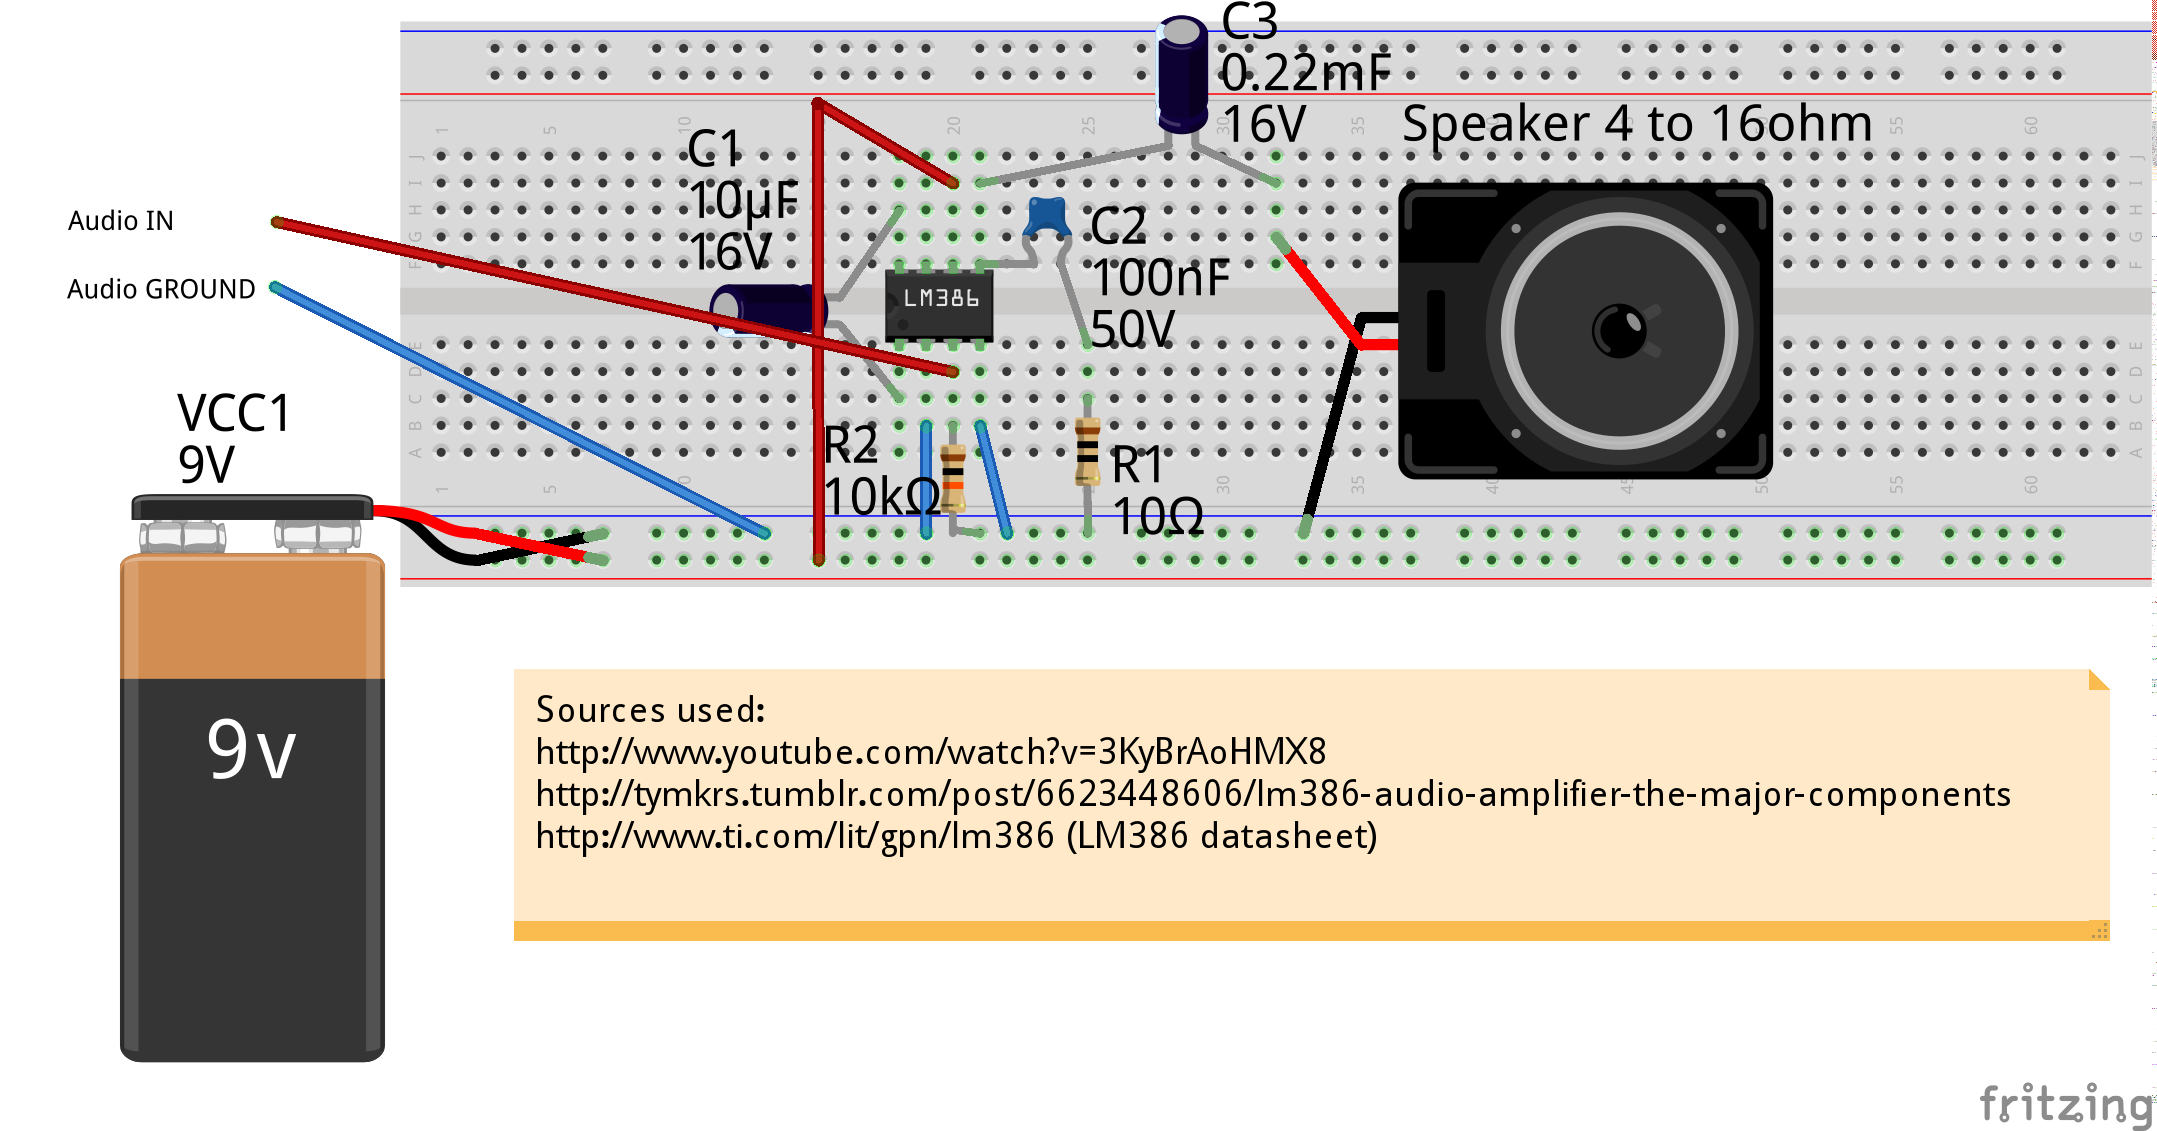
\includegraphics[scale=0.75]{audio_amplifier_lm386_bb.png}
    \caption{Breadboard view for the audio amplifier.}
  \end{center}
  \label{lm386_bb}
\end{figure}

In the heart of the audio amplifier stands the LM386 circuit, which is a "Low Voltage Audio Power Amplifier" and was more than enough for our use case. The figure in~\ref{lm386_bb} shows the breadboard view that we used used for the audio amplifier. The build is same to that what is shown on the LM386 datasheet, "amplifier with Gain = 200".

\begin{itemize}
  \item Between PINs 1 and 8 is a 10uF capacitor, which causes a gain on 200. In desibels this is around 20.
  \item PIN 2 is places to ground.
  \item PIN 3 takes the audio input, and is connected to ground through 10k ohm resistor.
  \item PIN 4 is placed to ground.
  \item PIN 5 is the amplified audio output.
  \item PIN 6 takes power
  \item PIN 7 is bybassed, doesn't take connection.
\end{itemize}

There weren't really any problems in assembling hardware, and everything with it worked as was planned.

\subsection{Motor control system}

Our motor control system consists of L293D motor control chip, 10k ohm resistor, battery case for two AA batteries and a small DC motor that has gears to lower main axis angular velocity. The parts are connected to each others as shown in figure \ref{l293d_bb}.

\begin{figure}
  \begin{center}
    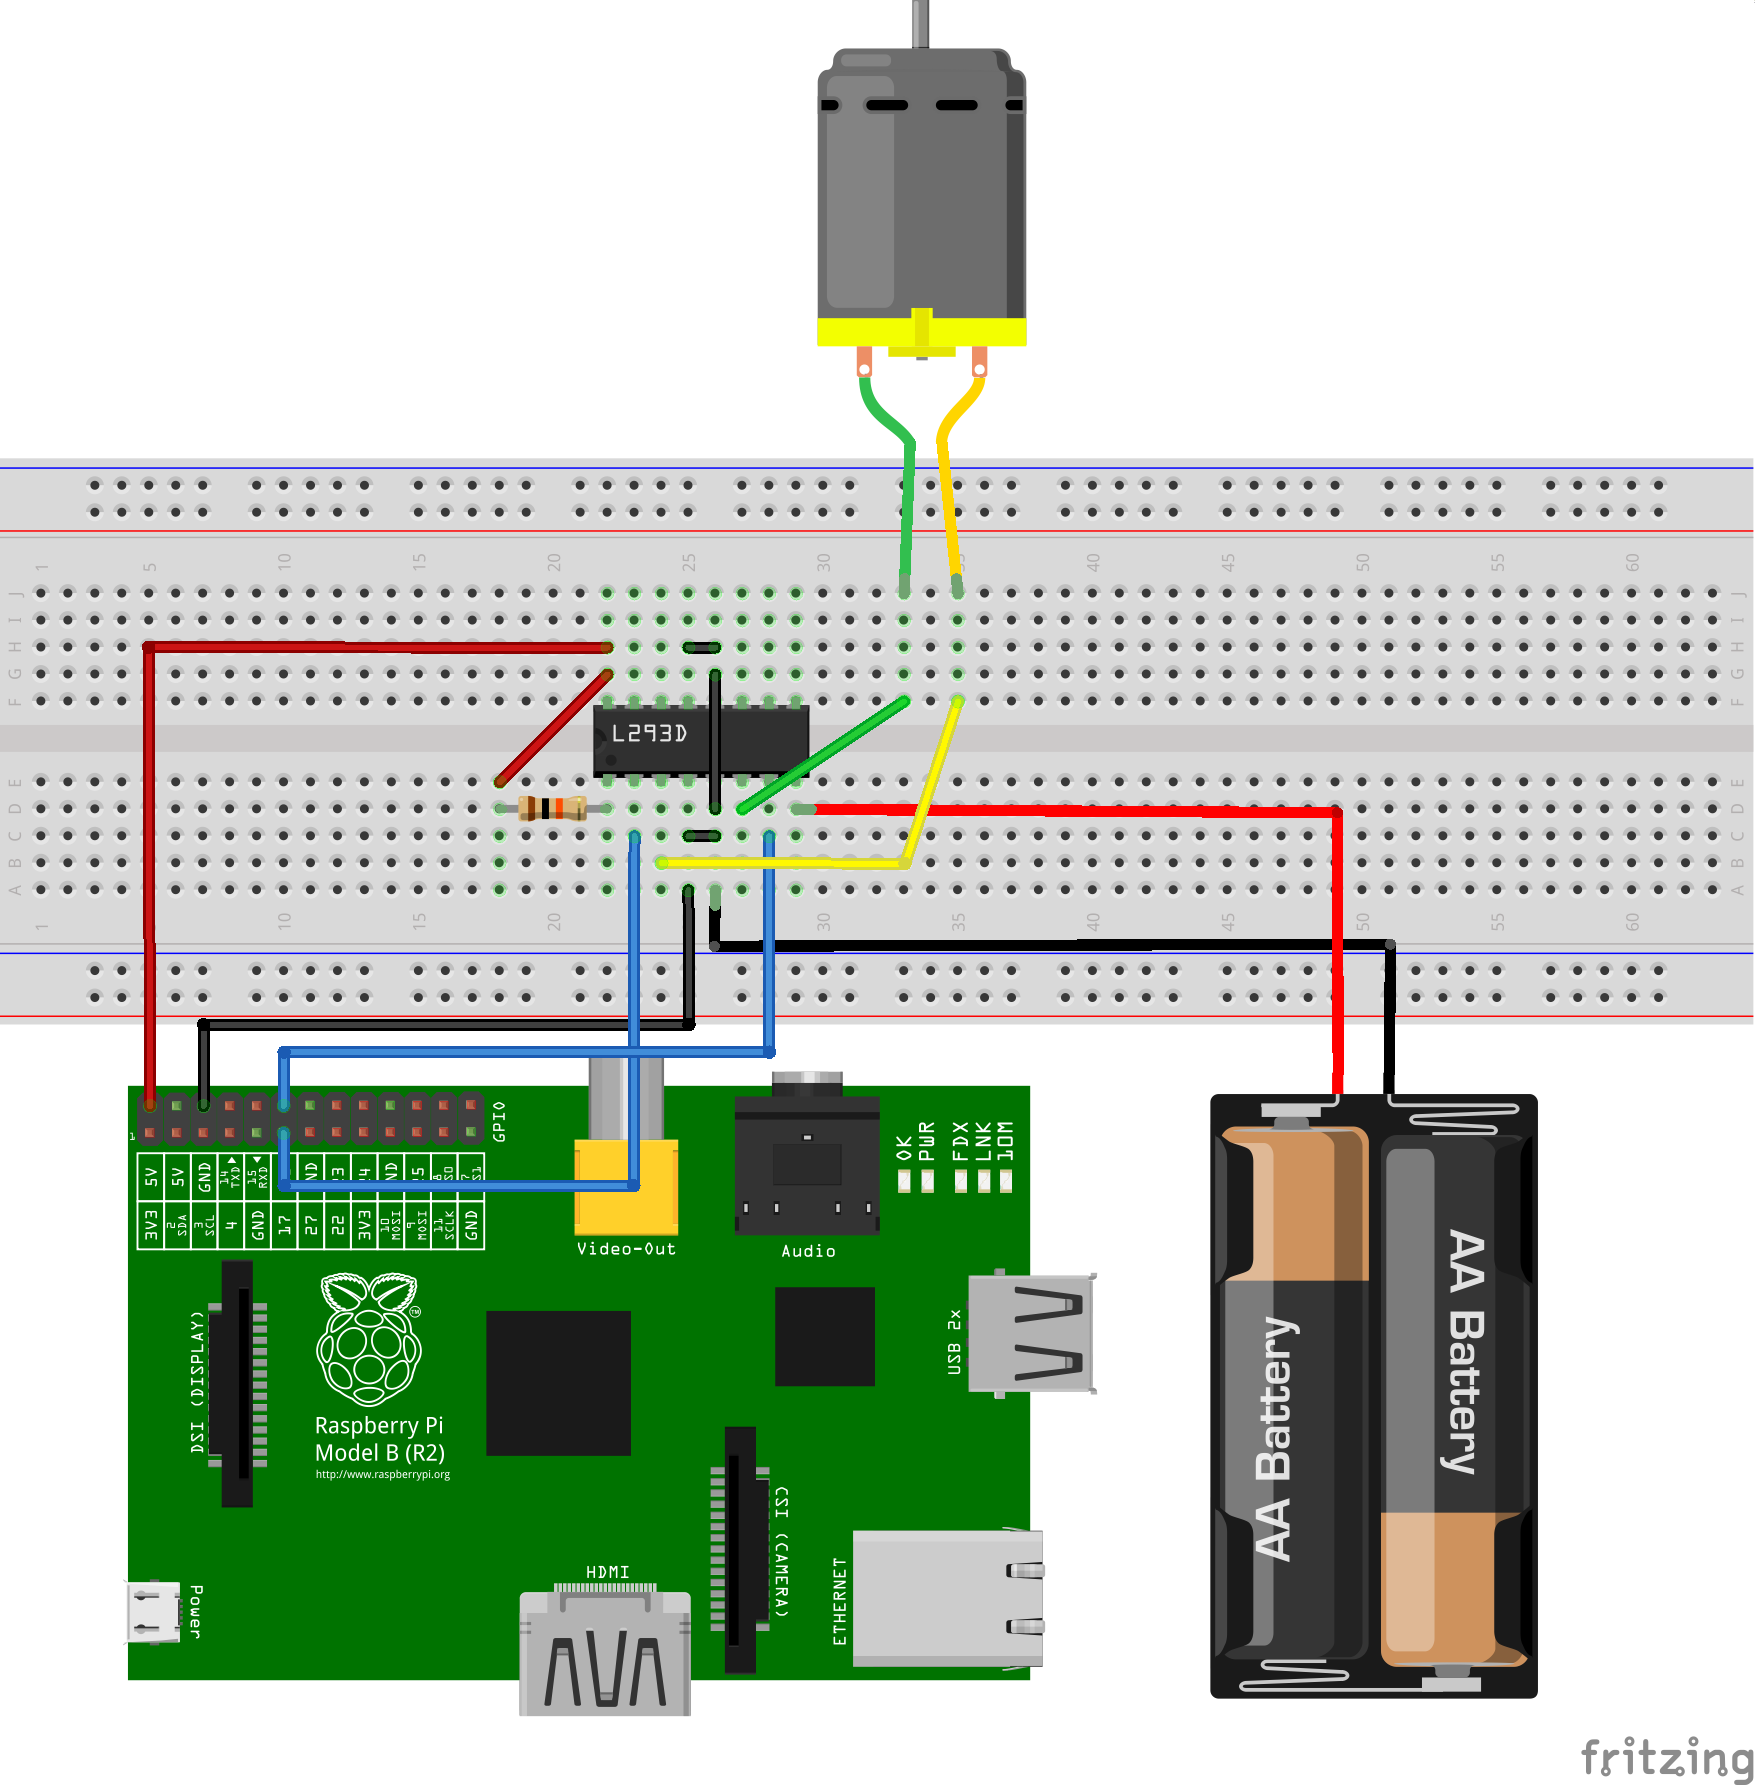
\includegraphics[scale=0.75]{motor_controllers_l293d_impl_bb.png}
    \caption{Breadboard view for motor controller.}
  \end{center}
  \label{l293d_bb}
\end{figure}

The L293D control chip gets it's operating power (VCC1) from Raspberry Pi 5V gpio pin. It also uses the same power through the transistor to send enable signal for motor controlling unit 1. The DC motor gets it's operating power from two AA batteries (3V) via L293D control chip's VCC2 pin.

\begin{table}
  \begin{center}
    \begin{tabular}{| l | l | l | l |}
      \hline
      Enable signal & Input 1A & Input 2A & Function \\ \hline
      H & L & H & Turn right \\ \hline
      H & H & L & Turn left \\ \hline
	  H & L & L & Stop \\ \hline
	  H & H & H & Stop \\ \hline
	  L & any & any & Stop \\ \hline
    \end{tabular}
    \caption{L293D chip's signal table. H = High, L = Low.}
  \end{center}
  \label{l293d_signal_table}
\end{table}

Raspberry Pi's GPIO pins 17 and 18 (hardware pins 11 and 12) high and low signals control the motor via L293D control chip. As shown in table \ref{l293d_signal_table}, the motor will rotate only when pin signals differ from each other. The enable signal is on at all times, since it is connected with a resistor to chip's VCC1.

\end{document}
